\chapter{Arduino}
Im Rahmen des Moduls wurde ein \emph{Internet of Things}-Applikation realisiert. Dafür wurde ein Arduino-Board sowie eine Reihe von Sensoren und Aktoren verwendet. Das Board, sowie die Sensoren und Aktoren sollen via Internet angesprochen werden.

Das Arduino ist ein \textbf{Mikrocontroller} mit einem 8-Bit-Prozessor und kann analoge und digitale Signale verarbeiten. Ein \textbf{Analogsignal} ist im Rahmen der Signaltheorie eine Form eines Signals mit stufenlosem und unterbrechungsfreiem Verlauf. Ein Analogsignal wird als glatte Funktion beschrieben. Ein \textbf{Digitalsignal} (von lat. digitus = Finger; mit Fingern wird gezählt) ist eine spezielle Form eines Signals, welches einen abgegrenzten und gestuften Wertvorrat umfasst und in der zeitlichen Abfolge nur zu bestimmten periodischen Zeitpunkten definiert ist bzw. eine Veränderung im Signalwert aufweist.

\begin{figure}[h!]
\centering
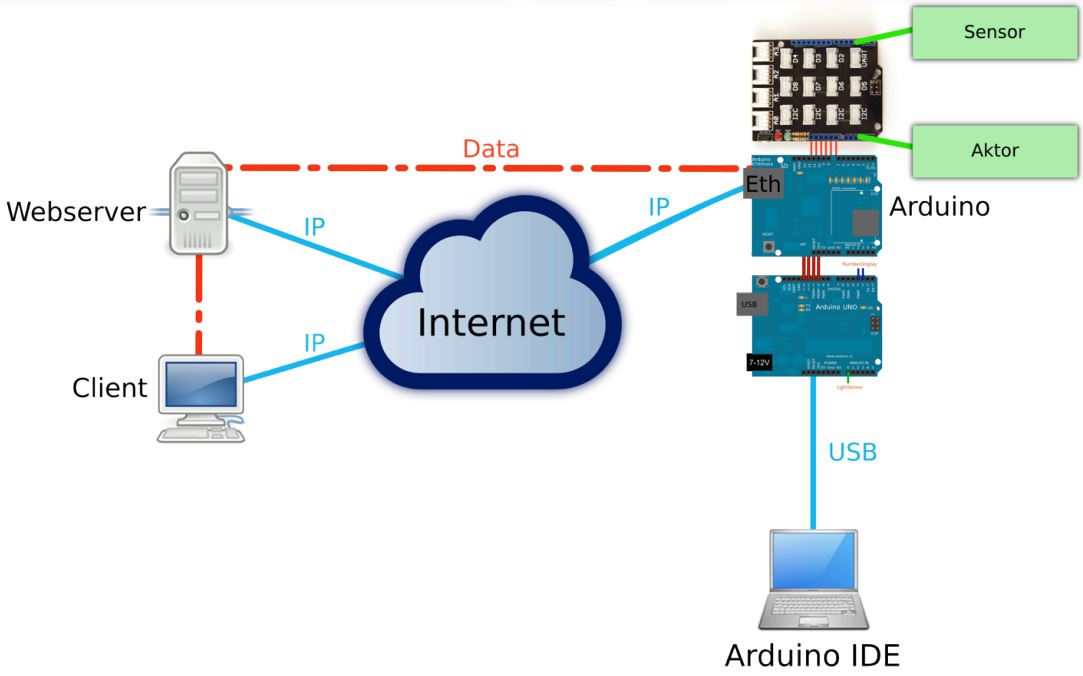
\includegraphics[width=0.7\linewidth]{fig/aruduino-projekt}
\caption{Projekt-Übersicht}
\label{fig:aruduino-projekt}
\end{figure}

\section{Architektur}
Projekte im IOT Bereich fordern immer eine Anbindung an ein Netzwerk. Die Werte die gemessen werden müssen publiziert oder abgerufen werden. Es gibt grundsätzlich zwei Arten:
\begin{description}
	\item[POLLING: Arduino als Server:] Der Arduino kann als REST-Server dienen. Er kann die Daten speichern und auf Anfrage ausliefern. Aber - Der Arduino ist eigentlich ein Mikroprozessor und solche Aufgaben sollten an andere Stelle delegiert werden. Dadurch können auch Steuersignale an den Server gesendet werden. (Achtung: Durch zu viel Pollen kann der Arduino überlastet werden.)
	\item[PUSH: Arduino als Client] Der Arduino schickt seine Daten an einen Server. Von da aus können die Daten beliebig ausgewertet werden. Viel bessere Variante. Wir belasten somit das Netzwerk nicht mit unnötigen Polls. Falls keine Verbindung zum Server aufgebaut werden kann, muss um die Persistenz gesorgt werden. Es können keine Steuersignale an den Server gesendet werden.
\end{description}

\section{Arduino Plattform}
Die Arduino Plattform besteht aus Hard- und Software (siehe Abbildung \ref{fig:aruduino-projekt}). Ermöglicht das Einbinden von Ansprechen von intelligenten Sensoren (vernetzte Sensoren). Die Daten können lokal (lokale Entscheidungen) oder an eine übergeordnet (übergeordnete Entscheidungen) ausgewertet werden. Als Grundlage dient das \textbf{Arduino-Board}, welches mit \emph{Shields} (steckbaren Aufsätzen) erweitert werden kann. Wir kennen folgende Shields:
\begin{description}
	\item[Grove (base shield)] Kann auf das Standard-USB-Board aufgesteckt werden und ermöglicht Steckverbindungen für Sensoren und Aktoren.
	\item[Ethernet Shield] Kann auch auf das Standard-USB-Board aufgesteckt werden und ermöglicht das Verbinden mit einem LAN (nutzt Arduino Ethernet Library).
\end{description}

\subsection{Sensoren}
\begin{description}
	\item[Grove - Button:] Ein Knopf worauf gedrückt werden kann.
	\item[Grove - Light Sensor:] Misst Intensität des Lichts. 
	\item[Grove - Barometer Sensor:] Druck messen.
	\item[Grove - I2C Color Sensor:] Misst Farbe des Umgebungslicht.
	\item[Grove - Moisture Sensor:] Misst Feuchtigkeit.
	\item[Grove - PIR Motion Sensor:] Sobald sich jemand in den Erkennungsbereich des Sensors bewegt geht der SIG Pin auf HIGH.
	\item[Grove - GPS:] Positionsbestimmung.
	\item[Grove - Touch Sensor:] Erkennt Berührung oder Nähe von menschlichen Fingern - Vier Berührungssensoren.
	\item[Last Sensor:] Gewichtssensor.
	\item[Digitaler Temperatur/Luftfeuchte Sensor DHT22 (RHT03):] Messung von Temperatur
	und relativer Luftfeuchtigkeit.
	\item[Grove - Air quality sensor:] Luft-Qualität messen.
	\item[Grove - sleep quality monitor:] GSR, standing for galvanic skin response, Detects strong emotions.
	\item[Grove - Infrared Receiver:] Empfängt IR Signale.
	\item[Grove - Serial Bluetooth:] Zugleich auch ein Aktor.
\end{description}

\subsection{Aktoren}
\begin{description}
	\item[Grove - 4-Digit Display:] 4 Zeichen rotes alpha-numerisches LED Display.
	\item[Grove - Infrared Emitter:] Sendet IR-Signale.
	\item[Grove - OLED Display:] Monochrom 128x64 Punkte Matrix Anzeige.
	\item[Grove - LED Bar:] 10 LED Segmente. Besteht aus einem roten, einem gelben, einem hellgrünen und sieben	grünen LEDs. Jedes Segment kann einzeln angesteuert werden.
\end{description}

\section{Sketch}
Entwickeln kann man in der Arduino IDE. Das Arduino wir per USB an den Rechner angeschlossen und kann somit relativ einfach die entwickelte Applikation deployen. Ein Arduino-Programme nennt man Sketch. Schlussendlich ist es nichts anders als C und C++. Einfach mit gewissen Eigenheiten. Beispielsweise gibt es eine vordefinierte Struktur, welches von jedem Sketch umgesetzt werden muss:

\begin{lstlisting}[language=C, caption=Sketch Struktur]
void setup() {
	// Wird nur einmal beim Start ausgeführt
}
void loop() {
	// Wird immer wieder ausgeführt
}
\end{lstlisting}

\subsection{Signale verwenden}
\begin{lstlisting}[language=C, caption=Signale verwenden]
// Pin-Mode setzen:
pinMode(); 		// INPUT, OUTPUT, INPUT_PULLUP

// Digital geht auf allen Pins
digitalRead(); 	// 0..1 = true,false = HIGH,LOW
digitalWrite(); // 0..1 = true,false = HIGH,LOW

// Nur auf A-Pins:
analogRead(); 	// 0..1023 ~= 0..5V, dauert 0.0001s

// Nur auf PWM-Pins:
analogWrite(); 	// PWM 0..255
\end{lstlisting}

\subsection{Beispiel Light Display}
\begin{itemize}
	\item Lesen des analogen Signals des Licht-Sensors.
	\item Schreiben der Werte auf das Number Display.
\end{itemize}

\begin{lstlisting}[language=C, caption=Light Display]
#include "TM1637.h"
#define CLK 2 // Port D2 on Grove Shield
#define DIO 3
#define LIGHT_PIN A0

TM1637 tm1637 = TM1637(CLK,DIO);
void setup() {
	tm1637.init();
	// BRIGHT_TYPICAL = 2, BRIGHT_DARKEST = 0, BRIGHTEST = 7;
	tm1637.set(BRIGHT_TYPICAL);
}

void loop() {
	delay(150);
	while(true)
	{
		int sensorValue = analogRead(LIGHT_PIN);
		tm1637.display(0, (int)(sensorValue / 1000));
		tm1637.display(1, (int)(sensorValue / 100)%10); 
		tm1637.display(2, (int)(sensorValue / 10)%10);
		tm1637.display(3, sensorValue % 10);
		delay(200);
	}
}
\end{lstlisting}

\subsection{Beispiel Rest Example - Arduino als Server}
\begin{lstlisting}[language=C]
#include <config_rest.h>
#include <rest_server.h>
#include <SPI.h>
#include <Ethernet.h>
#include <TM1637.h>

// Config of NumberDisplay
#define CLK 2 //pins definitions for TM1637 and can be changed to other ports       
#define DIO 3
#define SERVICES_COUNT  2

// Index of services in "service_get_pins" array
#define SERVICE_LIGHTSENSOR 0
#define SERVICE_DISPLAY 1
#define LIGHTPIN A0
#define CRLF "\r\n"

// Enter a MAC address and IP address for your Arduino below.
// The IP address will be dependent on your local network:
byte mac[] = { 0x90, 0xA2, 0xDA, 0x00, 0x68, 0xF8 };
byte ip[] = { 192, 168, 2, 200 };
byte gateway[] = { 192, 168, 2, 1 };
byte subnet[] = { 255, 255, 255, 0 };

// Start a TCP server on port 7999
EthernetServer server(80);

// Create instance of the RestServer
RestServer request_server = RestServer(Serial);

TM1637 tm1637(CLK,DIO);

// method that register the resource_descriptions with the request_server
// it is important to define this array in its own method so that it will
// be discarted from the Arduino's RAM after the registration.
void register_rest_server() {
	resource_description_t lightsensor = { "output_light", false, { 0, 1023 } };
	resource_description_t numberdisplay = { "input_numberdisplay", true, { 0, 9999 } };
	
	resource_description_t resource_description[SERVICES_COUNT];
	resource_description[SERVICE_LIGHTSENSOR] = lightsensor;
	resource_description[SERVICE_DISPLAY] = numberdisplay;
	request_server.register_resources(resource_description, SERVICES_COUNT);
}

void setup() {
	// start the Ethernet connection and the server:
	Ethernet.begin(mac, ip, gateway, subnet);
	
	// setup NumberDisplay
	tm1637.init();
	//BRIGHT_TYPICAL = 2, BRIGHT_DARKEST = 0, BRIGHTEST = 7;
	tm1637.set(BRIGHT_TYPICAL); 
	
	// manually initialize input and output pins, if not done by a library
	pinMode(LIGHTPIN, INPUT);
	
	server.begin();	
	// register resources with resource_server
	register_rest_server();
}

void loop() {
	// listen for incoming clients
	EthernetClient client = server.available();
	
	// CONNECTED TO CLIENT
	if (client) {
		while (client.connected()) {			
			// get request from client, if available
			if (request_server.handle_requests(client)) {
				read_write_data();
				request_server.respond();       // tell RestServer: ready to respond
			}			
			// send data to client, when ready      
			if (request_server.handle_response(client))
			break;
		}
		// give the web browser time to receive the data and close connection
		delay(1);
		client.stop();
	}
}

void read_write_data() {
	for (int j = 0; j < SERVICES_COUNT; j++) {
		if (!request_server.resource_post_enabled(j)) {
			if (j == SERVICE_LIGHTSENSOR) {
				request_server.resource_set_state(j, analogRead(LIGHTPIN));
			}
		}
		if (request_server.resource_post_enabled(j)) {
			if (j == SERVICE_DISPLAY) {
				setNumberDisplay(request_server.resource_get_state(j));
			}
			// Or e.g. for analog PINS
			// analogWrite(service_pins[j], request_server.resource_get_state(j));
		}
	}
}

void setNumberDisplay(int value) {
	tm1637.display(0, (int) (value / 1000));
	tm1637.display(1, (int) (value / 100) % 10);
	tm1637.display(2, (int) (value / 10) % 10);
	tm1637.display(3, value % 10);
}
\end{lstlisting}


% Themen:
% done Grundlegende Konzepte der Arduino Plattform
% done Arduino Sensoren und Aktoren
% done Entwicklungsumgebung
% done Arduino Programmierung und Einbindung in eine IoT Applikation.

% Dokumente: 
% done 08 AITEC-Projekt.pdf
% done 04 Einführung Arduino Plattform.pdf
% done 04 Arduino Entwicklungsumgebung.pdf